
\documentclass[a4paper,12pt]{report}
\usepackage{graphicx}
\usepackage{subfig}

\begin{document}

\begin{figure}[!tbp]
    \centering
    \subfloat{
\includegraphics[width=0.5\textwidth]{logo_ueh.jpg}\label{fig:logo_ueh}}
    \hfill
    \subfloat{
\includegraphics[width=0.4\textwidth]{logoFDS.jpg}\label{fig:logoFDS}}
\end{figure}

\begin{figure}[h]
    \centering
    
\includegraphics[width=1\textwidth]{lib}
    \label{image-lib}
\end{figure}


\title{BiblioTech \\ Automatisation de la Gestion des prêts au sein d'une Bibliothèque universitaire \\ par:}
\author{ALTIDOR Jean-Bernard T. \\ DUBUCHE Kevin J. \\ THEODORE Barbara G.}
\date{Décembre 2020}
\maketitle

\paragraph{}
\textbf{\underline{Projet de Génie Logiciel}} \par 
\textit{Professeur} : M. Faubert Étienne \par 
\textit{Classe} : 3ème année \par 
\textit{Section} : Électronique \par 
\textit{Promotion} : 2019-2020

\tableofcontents

\chapter*{}
\section*{Resume}
Une bibliothèque universitaire souhaite automatiser
sa gestion

\section*{Glossaire}
Termes pourvant porter a confusion
Lorem ipsum dolor sit amet, consectetur adipiscing elit. Mauris at ultrices purus. Donec finibus metus et augue sodales posuere. Proin sit amet turpis dictum, iaculis felis in, scelerisque massa. Nullam aliquam nunc eget fringilla volutpat. Integer et mauris et massa imperdiet scelerisque mollis at sapien. Donec condimentum felis eget sagittis ultricies. Nunc laoreet augue id consectetur vulputate. Cras sagittis aliquam risus sit amet tempus. Curabitur finibus neque eget magna efficitur, sed dignissim quam sagittis. Ut euismod justo id gravida pulvinar. Ut urna magna, auctor maximus volutpat ac, elementum sed mi.


\chapter{Contexte}
    \section{Fonctionnenment d'une bibliothèque}
\paragraph{}
De façon générale, les prêts au sein d'une bibliothèque
exige la présence de grand nombre de ressources. En se 
basant directement sur la réalité liée à une entité
universitaire, le processus est le suivant: \par 
\begin{enumerate}
    \item Un étudiant désire faire un prêt.
    \item Il se rend à la bibliothèque.
    \item L'étudiant fait sa demande.
    \item Le responsable va vérifier si le livre demandé est disponible.
    \begin{itemize}
        \item[*] Si le livre est disponible, le responsable enregistre le prêt 
        et le donne au demandeur.
        \item[*] Si le livre n'est pas disponible, il l'en informe.
    \end{itemize} 
    \item L'étudiant s'en va avec ou sans livre.
\end{enumerate}

    \section{Affluence résultante}
\paragraph{}
Un tel processus pourrait avoir des conséquences négatives
sur le fonctionnement de la bibliothèque. Pour commencer, cela pourrait
être irritant pour un étudiant de faire un déplacement inutile
dans le but d'emprunter un livre et ne pas le trouver. De plus, 
il se pourrait que plusieurs étudiants aient besoin de divers livres
au même instant. Le comble pour le responsable sera de desservir tout 
un groupe. Non seulement l'affluence pourrait nuire au calme demandé
dans un tel espace, mais cela fatiguerait rapidement le bibliothécaire.
    
    \section{Avantages portées par la numérisation}
\paragraph{}
Grâce à la numérisation du système de gestion des prêts,
il deviendra possible pour un intéressé de faire des consultations
en ligne. Ceci diminuerait tant les déplacements inutiles que les 
affluences. En plus, certaines tâches pourraient facilement être 
automatisées, ce qui aiderait à limiter les erreurs humaines.   
\paragraph{}
Dans le souci d'assurer la faciliter une eventuelle expansion du projet ou handover, nous laissons à la disposition de l'équipe en fontion la méthodologie utilisée pour la réalisation du dit projet.

\chapter{Organisation}
        \section{Approche de travail}
\paragraph{}
Afin de réaliser au mieux ce travail, nous avons quelque peu respecté la methode agile,
nous permettanat alors de revenir en arrière en cas de souci. Il est vrai que nous
n'avons pas gardé un rapport étroit avec notre client. Néanmoins, nous avons respecté 
les autres contraintes liées à la méthodologie indiquée.
        \section{Methodologie}
        Lorem ipsum dolor sit amet, consectetur adipiscing elit. Mauris at ultrices purus. Donec finibus metus et augue sodales posuere. Proin sit amet turpis dictum, iaculis felis in, scelerisque massa. Nullam aliquam nunc eget fringilla volutpat. Integer et mauris et massa imperdiet scelerisque mollis at sapien. Donec condimentum felis eget sagittis ultricies. Nunc laoreet augue id consectetur vulputate. Cras sagittis aliquam risus sit amet tempus. Curabitur finibus neque eget magna efficitur, sed dignissim quam sagittis. Ut euismod justo id gravida pulvinar. Ut urna magna, auctor maximus volutpat ac, elementum sed mi.
        \section{Repartition des taches}
        Lorem ipsum dolor sit amet, consectetur adipiscing elit. Mauris at ultrices purus. Donec finibus metus et augue sodales posuere. Proin sit amet turpis dictum, iaculis felis in, scelerisque massa. Nullam aliquam nunc eget fringilla volutpat. Integer et mauris et massa imperdiet scelerisque mollis at sapien. Donec condimentum felis eget sagittis ultricies. Nunc laoreet augue id consectetur vulputate. Cras sagittis aliquam risus sit amet tempus. Curabitur finibus neque eget magna efficitur, sed dignissim quam sagittis. Ut euismod justo id gravida pulvinar. Ut urna magna, auctor maximus volutpat ac, elementum sed mi.


\chapter{Implémentation}
        \section{Choix des technologies}
\paragraph{}   
\begin{tabular}{|c|p{2.7cm}|p{6cm}|}
        \hline
        Technologie & Utilité & Raison du choix \\
        \hline
        Linux & OS & Les trois membres utilisent Linux \\
        \hline
        Github & Système de contrôle de version & Il permet de travailler à distance et en même temps et de garder une trace des différentes versions\\
        \hline 
        StarUml & Conception & Le choix de UML a été imposé par le client dès le départ. \\
        \hline
        (you know better) & Programmation web & Donne la raison \\
        \hline
\end{tabular}
\par 

\section{La hiérarchie dans l'application}
\paragraph{}
Trois niveaux d'utilisation sont considérés au sein de l'application.
Chacun d'eux détient des privilèges en plus de celui qui vient directement après lui.
Les abonnés sont ceux qui peuvent poser le moins d'actions possibles dans le système. ils 
ne peuvent rien faire de plus que lire les données disponibles. De ce fait, 
ils peuvent voir tous les livres qui sont disponibles à chaque instant, et recevoir 
des notifications lorsqu'ils auront passé trop de temps avec un ouvrage en main.\par 
De leur côté, les bibliothécaires détiennent des droits de ressources matérielles. En plus
des droits d'accès des abonnés, ils peuvent agir sur les différents 
emprunts ainsi que que sur les données relatives aux ouvrages. \par 
Et enfin, le gestionnaire peut tout faire, et plus particulièrement gérer les 
utilisateurs du système.
\section{Interface utilisateur}
\paragraph{}       
L'interface utilisateur a été réfléchi de telle sorte que n'importe qui 
peut se retrouver facilement sur l'application. Aucun téléchargement préalable n'est requis, de même 
qu'il ne sera pas du tout nécessaire de faire un cours complet pour expliquer à un nouvel utilisateur
les différentes utilités de chaque bouton.

\section{Diagrammes}
\subsection{Diagrammes des cas d'utilisation}
\paragraph{} 
Lorem ipsum dolor sit amet, consectetur adipiscing elit. Mauris at ultrices purus. Donec finibus metus et augue sodales posuere. Proin sit amet turpis dictum, iaculis felis in, scelerisque massa. Nullam aliquam nunc eget fringilla volutpat. Integer et mauris et massa imperdiet scelerisque mollis at sapien. Donec condimentum felis eget sagittis ultricies. Nunc laoreet augue id consectetur vulputate. Cras sagittis aliquam risus sit amet tempus. Curabitur finibus neque eget magna efficitur, sed dignissim quam sagittis. Ut euismod justo id gravida pulvinar. Ut urna magna, auctor maximus volutpat ac, elementum sed mi.
\subsection{Diagrammes de séquence}
\paragraph{} 
Lorem ipsum dolor sit amet, consectetur adipiscing elit. Mauris at ultrices purus. Donec finibus metus et augue sodales posuere. Proin sit amet turpis dictum, iaculis felis in, scelerisque massa. Nullam aliquam nunc eget fringilla volutpat. Integer et mauris et massa imperdiet scelerisque mollis at sapien. Donec condimentum felis eget sagittis ultricies. Nunc laoreet augue id consectetur vulputate. Cras sagittis aliquam risus sit amet tempus. Curabitur finibus neque eget magna efficitur, sed dignissim quam sagittis. Ut euismod justo id gravida pulvinar. Ut urna magna, auctor maximus volutpat ac, elementum sed mi.
\subsection{Diagrammes de ce ce qu'on a demande}
\paragraph{} 
Lorem ipsum dolor sit amet, consectetur adipiscing elit. Mauris at ultrices purus. Donec finibus metus et augue sodales posuere. Proin sit amet turpis dictum, iaculis felis in, scelerisque massa. Nullam aliquam nunc eget fringilla volutpat. Integer et mauris et massa imperdiet scelerisque mollis at sapien. Donec condimentum felis eget sagittis ultricies. Nunc laoreet augue id consectetur vulputate. Cras sagittis aliquam risus sit amet tempus. Curabitur finibus neque eget magna efficitur, sed dignissim quam sagittis. Ut euismod justo id gravida pulvinar. Ut urna magna, auctor maximus volutpat ac, elementum sed mi.
\subsection{Diagrammes de ce qu'on n'a pas demande}
\paragraph{} 
Lorem ipsum dolor sit amet, consectetur adipiscing elit. Mauris at ultrices purus. Donec finibus metus et augue sodales posuere. Proin sit amet turpis dictum, iaculis felis in, scelerisque massa. Nullam aliquam nunc eget fringilla volutpat. Integer et mauris et massa imperdiet scelerisque mollis at sapien. Donec condimentum felis eget sagittis ultricies. Nunc laoreet augue id consectetur vulputate. Cras sagittis aliquam risus sit amet tempus. Curabitur finibus neque eget magna efficitur, sed dignissim quam sagittis. Ut euismod justo id gravida pulvinar. Ut urna magna, auctor maximus volutpat ac, elementum sed mi.


\section{Diagrammes incontournables}
\subsection{Diagramme d’activité du processus de Gestion des prêts dans la bibliothèque}
\paragraph{}
\begin{figure}[h]
        \centering
        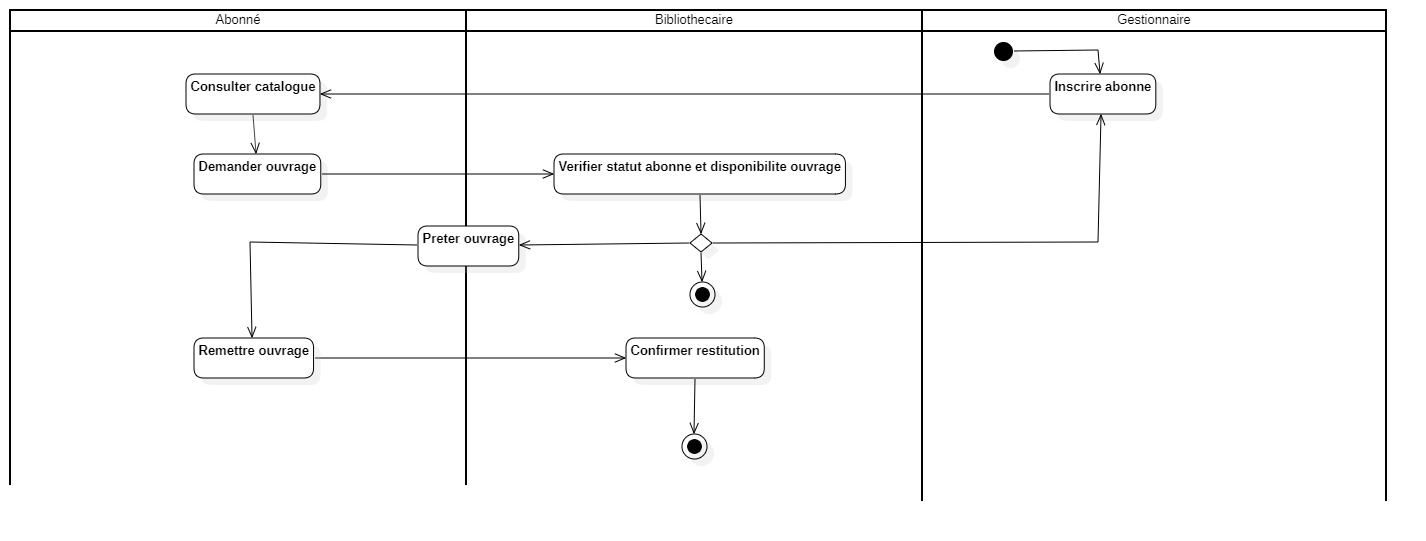
\includegraphics[width=1\textwidth]{ActivityDiagram1}
        \caption{Diagramme d’activité du processus de Gestion des prêts dans la bibliothèque}
        \label{image-ActivityDiagram1}
        \end{figure}
\par
Les prêts au sein de la bibliothèque universitaire suivent un ensemble d'étapes précis.
Certaines contraintes sont donc à respecter continuellement. Pour commencer, n'importe qui 
peut consulter la liste des ouvrages accessibles dans la biblio. Mais pour savoir quel 
ouvrage est disponible au moment de la recherche, il faut que le gestionnaire enregistre 
l'abonné. De son côté, il faut que le bibliothécaire enregistre les ouvrages acquis 
dans la base de données du système. \par 
Après s'être assuré de la disponibilité d'un livre, l'abonné peut alors se rendre sur 
place pour effectuer l'emprunt. Du coup, le bibliothèque a pour responsabilité de relever
toutes les informations relatives à l'emprunt en question. Certains champs sont obligatoires
et le système renverra un message d'erreur s'ils ne sont pas remplis. Si l'abonné a déjà 
trois livres en sa possession, le système n'autorise pas la validation de l'emprunt.
Une fois l'emprunt validé, l'abonné peut vaquer à ses occupations sans problème. Il lui 
est donné trois semaines pour rester en possession du livre. De façon exceptionnelle, il 
peut pourtant le garder durant cinq semaines. Pourtant, une fois ce délai atteint, le 
système envoie une relance automatique sur le mail du concerné pour le rappeler qu'il doit 
rapporter ce livre en question.
Lorsque l'abonné rend le livre, il se présente encore une fois à la bibliothèque et le 
responsable se charge de modifier l'emprunt en y ajoutant une date de restitution. \par 
Ainsi se déroule le cycle de la gestion des emprunts au sein de la bibliothèque.
\subsection{Diagramme de classe de gestion des prêts}
\paragraph{}

Ce diagramme est utile pour présenter les différentes classes ainsi que les relations 
entre elles. Il est obligatoire lors d'une modélisation. Selon certaines sources, il 
s'agit d'un document indispensable sui représente la vue de conception statique 
d'un système. Il serait donc impensable de concevoir l'application sans prendre le temps 
d'implémenter cet outil.
\par 
Il se présente de la sorte: \par 
\begin{figure}[h]
        \centering
        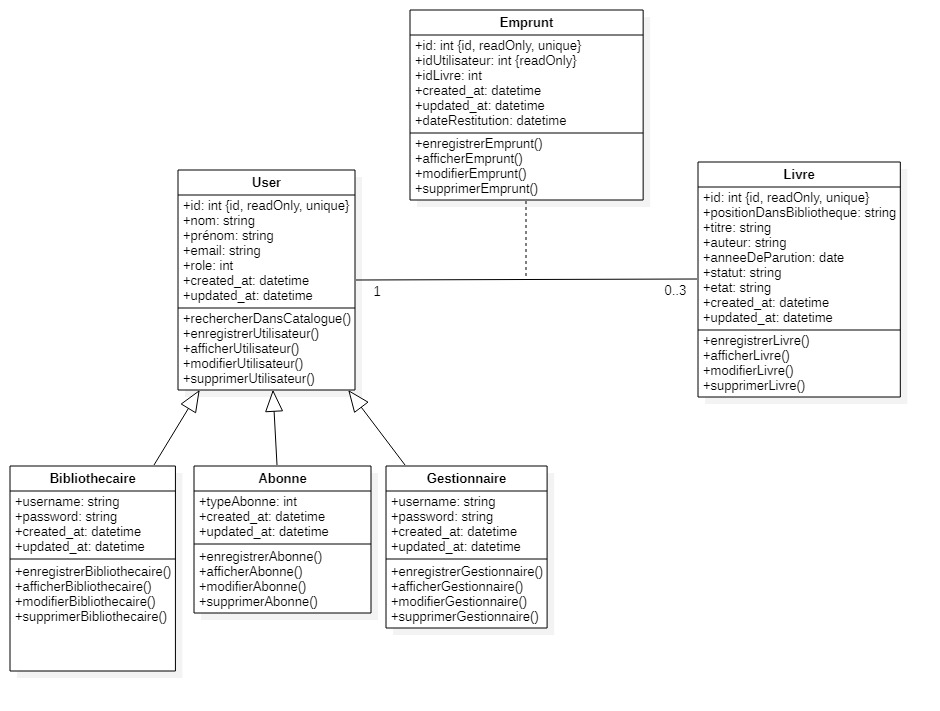
\includegraphics[width=1\textwidth]{ClassDiagram1}
        \caption{Diagramme de classe de gestion des prêts}
        \label{image-ClassDiagram1}
        \end{figure}
\par

\chapter{Conclusion}
\paragraph{}
L'implémentation de cette application est à la fois bénéfique pour le gestionnaire,
le bibliothécaire et l'abonné. La disponibilité du catalogue permet à l'abonné de 
se renseigner sur les livres disponibles sans faire de déplacement. De son côté, le 
bibliothécaire peut retracer les ouvrages en tout temps. Et enfin, le gestionnaire n'aura 
point l'obligation de traquer les abonnés n'ayant pas encore remis un ouvrrage
puisque la relance se fait de manière automaatique.   

\end{document}